\documentclass{article}
\usepackage{amsmath, amssymb, amsthm}
\usepackage{geometry}
\usepackage{enumitem}
\usepackage{xcolor}
\usepackage{listings}
\usepackage{bm}
\usepackage{graphicx}

\usepackage[ruled,vlined]{algorithm2e}

\geometry{a4paper, margin=1in}

\lstset{
    language=Python,
    basicstyle=\ttfamily\footnotesize,
    keywordstyle=\color{blue},
    stringstyle=\color{green},
    commentstyle=\color{gray},
    numbers=left,
    numberstyle=\tiny\color{gray},
    stepnumber=1,
    numbersep=5pt,
    showspaces=false,
    showstringspaces=false,
    breaklines=true,
    frame=single,
    captionpos=b
}

\newcommand{\py}[1]{\texttt{\lstinline!#1!}}

\title{Additional material Week 3}

\begin{document}
\maketitle
\section{Question 1}
\subsection{Statement}
Perform linear regression between the Buildup Index (BUI) and the Fire Weather Index (FWI) in The Algerian Forset Dataset.

\subsection{Theory}
We want to model the relation between an independent variable $x$ and a dependent variable $y$ with a line $y=mx+q$,
where $m$ is the slope of the line and $q$ is its $y$-intercept.

To find the best-fitting line, we use the method of least squares, which minimizes the sum of squared residuals, i.e. the difference between observed and predicted values:
\begin{equation*}
    E = \sum_{i=1}^n r_i^2 = \sum_{i=1}^n (\widehat{y_i} - y_i)^2
\end{equation*}

Setting the derivative of $E$ with respect to $m$ and $q$ to zero, the following formulas for $m$ and $q$ are found:
\begin{align*}
    \hat{m} = \frac{n \sum\limits_{i=1}^n x_i y_i - \sum\limits_{i=1}^n x_i \sum\limits_{i=1}^n y_i}{ n \sum\limits_{i=1}^n x_i^2 - \left( \sum\limits_{i=1}^n x_i \right)^2} \\
    \hat{q} = \frac{\sum\limits_{i=1}^n y_i - \hat{m} \sum\limits_{i=1}^n x_i}{n}
\end{align*}

\subsection{Python solution}
We just need to use the same code that we used during the lecture, extracting the BUI from the dataset with \py{x = my_dataset["BUI"].value}.
Listing \ref{q1pycode} shows the final Python code for the solution.
\lstinputlisting[language=Python, caption={Python code solution for the Question}, label=q1pycode]{W2_Q1_BUI_FWI.py}

\subsection{Matlab solution}
We just need to use the same code that we used during the lecture, extracting the BUI from the dataset with \py{x = my_dataset.BUI}.
Listing \ref{q1matcode} shows the final Matlab code for the solution.
\lstinputlisting[language=Matlab, caption={Matlab code solution for the Question}, label=q1matcode]{W2_Q1_BUI_FWI.m}

\subsection{Comments}
\begin{figure}[h]
\centering
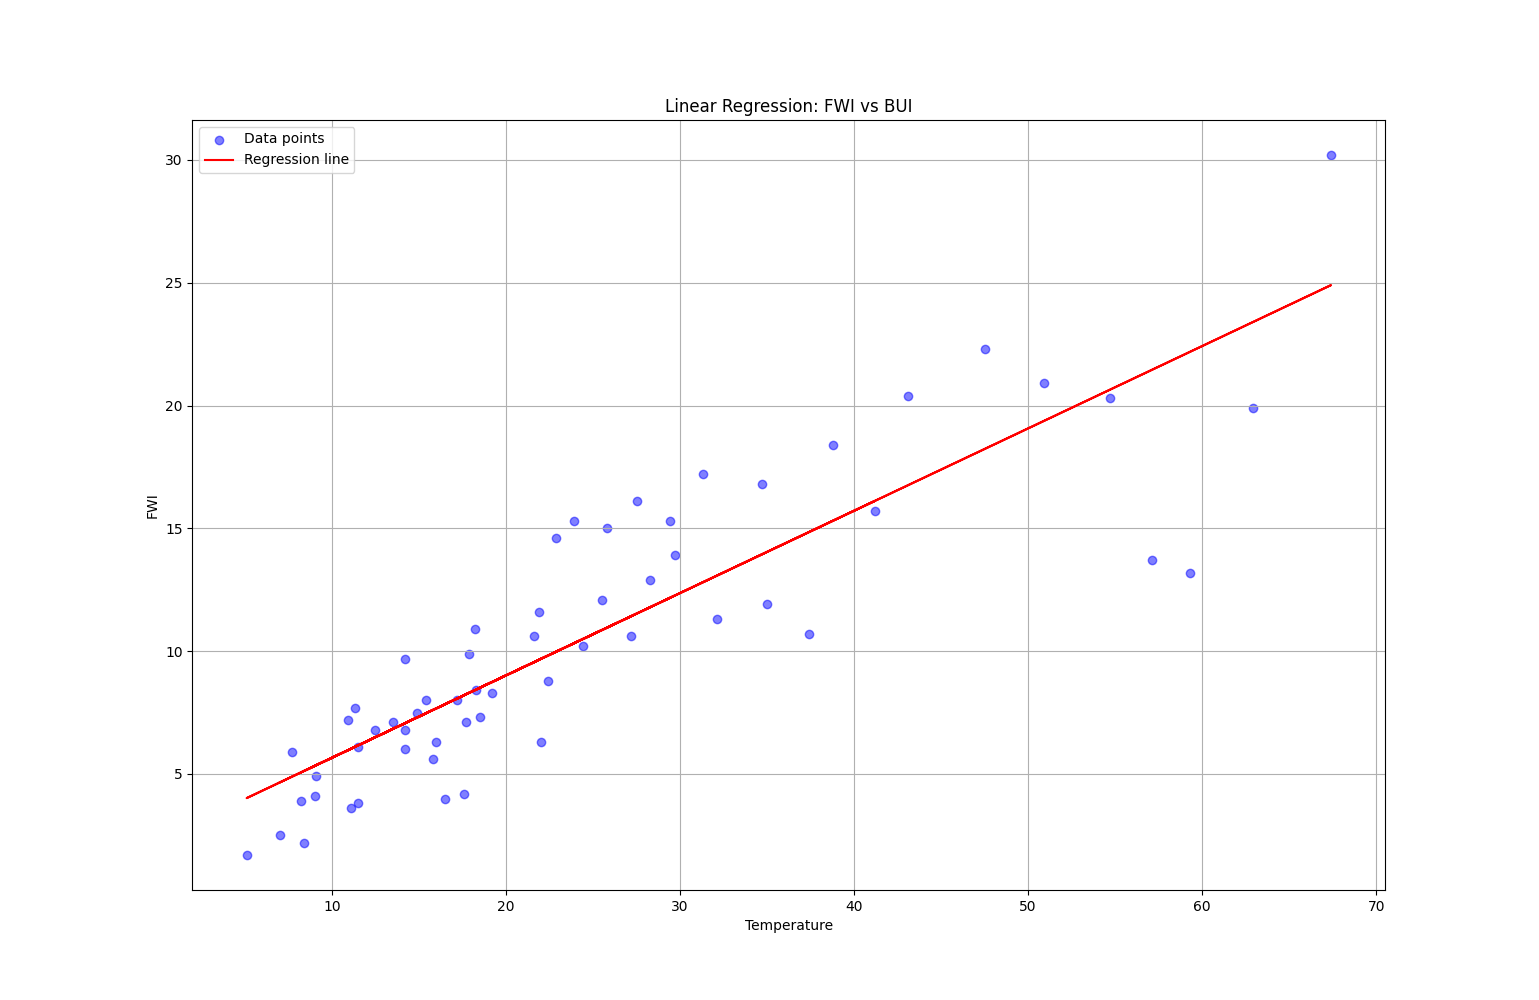
\includegraphics[width=0.7\linewidth]{W2_Q1_BUI_plot.png}
\caption{\label{fig:BUI_plot} BUI-FWI dataset points in blue, and corresponding regression line in red.}
\end{figure}
We can see from the value of the regression line slope \py{m = 0.3353} and from the graph in Figure \ref{fig:BUI_plot} that the correlation between BUI and FWI is positive. This is unsurprising: the Buildup Index measures the amount of fuel available in the environment, so higher BUI means that fires spread more easiliy once they start, corresponding to higher fire risk.

\section{Question 2}
\subsection{Statement}
Linear regression can always produce a fitting line given a set of data points $(x_i, y_i)$. How can we assess how well is the regression line fitting the available data? Compute the coefficient of determination $R^2$ for temperature-FWI, RH-FWI and BUI-FWI linear reagressions in the Algerian forest dataset and evaluate which one of them has the best fit.

\subsection{Theory}
The most straightforward way to evaluate the goodness of the fit is to examine the \emph{sum of the squares of the residuals}, which we denoted with $E$ and is the "score" that we minimized to find the line in the first place:
\begin{equation*}
    E = \sum_{i=1}^n r_i^2 = \sum_{i=1}^n (\widehat{y_i} - y_i)^2
\end{equation*}

In general, the lower the value of $E$, the better the fit. However, the absolute value of $E$ depends on the scaling of the variables involved: scaling the dataset up will increase $E$, even though intuitively the goodness of the fit should remain the same. This makes it difficult to directly compare models with different units or scales.  

To address this, we standardize the residuals, which requires computing a reference value. In practice we choose the \emph{total sum of squares} $\bar{E}$, defined as the sum of the squared differences between the $y$ values and their means $\bar{y} = \frac{1}{n}\sum_{i=1}^{n} y_i$.
\begin{equation*}
    \bar{E}=\sum_{i=1}^{n} (y_i -\bar{y})^2
\end{equation*}

$\bar{E}$ represents the variance intrinsic to the data; moreover, it can be seen as the "score" $E$ associated with a baseline regression model with $m=0, q=\bar{y}$, that is a model that always predicts the same value, equal to the mean of the dataset, no matter the input $x_i$. 
Then, the \emph{coefficient of determination} $R^2$ is defined as:
\begin{equation*}
    R^2 = 1 - \frac{E}{\bar{E}}
\end{equation*}

$R^2$ is always a value between 0 and 1: lower values indicate a poor fit, viceversa higher  ones indicate a good fit. The worst case $R^2 =0 $ corresponds to the baseline model that we just discussed ($E = \bar{E}$), while the best case scenario $R^2 =1 $ corresponds to a perfect fit, where the regression line interpolates all the data points without errors ($E = 0$).

$R^2$ can also be interpreted as the \emph{fraction of explained variance} of the model, i.e. how much of the intrinsic variance of the dataset $\bar{E}$ is captured by the model, versus how much of it is left unexplained.

\subsection{Python solution}
To compute the coefficient of determination for our dataset, we need to compute $E$ and $\bar{E}$ explicitly; to do this, we can use the concept of \emph{vectorized operations} that we learned during the lecture. In particular, we use the fact that adding a constant to a vector or multiplying it by a constant is treated in a vectorized manner, i.e.  the operation is applied to all terms of the array.

We will define a function for each term: for $\bar{E}$ we first need to compute the mean $\bar{y}$, while for the error $E$ we need the predicted values $\widehat{y_i} = \hat{m} x_i + \hat{q}$.
\lstinputlisting[language=Python, firstline=18, lastline=27]{W2_Q2_r_squared.py}

The mean $\bar{y}$ can also be computed directly with the \py{np.mean} function: \py{y_bar = np.mean(y)}.
Finally, we write one last function applying the definition of $R^2$.
\lstinputlisting[language=Python, firstline=29, lastline=33]{W2_Q2_r_squared.py}

Listing \ref{q2pycode} shows the final Python code for the solution.
\lstinputlisting[language=Python, caption={Python code solution for the Question}, label=q2pycode]{W2_Q2_r_squared.py}

\subsection{Matlab solution}
To compute the coefficient of determination for our dataset, we need to compute $E$ and $\bar{E}$ explicitly; to do this, we can use the concept of \emph{vectorized operations} that we learned during the lecture. In particular,adding a constant to a vector and multiplying it by a constant are treated in a vectorized manner, i.e. the opration is applied to all terms of the array. To specify that an operation should be vectorized, remember to put the \py{.} before it.

We will define a function for each term: for $\bar{E}$ we first need to compute the mean $\bar{y}$, while for the error $E$ we need the predicted values $\widehat{y_i} = \hat{m} x_i + \hat{q}$.
\lstinputlisting[language=Matlab, firstline=1, lastline=10]{W2_Q2_r_squared.m}

The mean $\bar{y}$ can also be computed directly with the \py{mean} function: \py{y_bar = mean(y);}.
Finally, we write one last function applying the definition of $R^2$.
\lstinputlisting[language=Matlab, firstline=12, lastline=16]{W2_Q2_r_squared.m}

Listing \ref{q2matcode} shows the final Matlab code for the solution.
\lstinputlisting[language=Matlab, caption={Matlab code solution for the Question}, label=q2matcode]{W2_Q2_r_squared.m}

\subsection{Comments}
\begin{lstlisting}[language=python]
    Coefficient of determination for Temperature-FWI regression: 0.33059760059566334
    Coefficient of determination for RH-FWI regression: 0.1647176771914015
    Coefficient of determination for BUI-FWI regression: 0.7540921186111107
\end{lstlisting}

The coefficient of determination is a measure of the goodness of fit. In practice, a better fit is often interpreted as a stronger, more significant correlation existing between the quantities we are considering; this may hint at some underlying meachanism that links the variables together. 
Among the 3 $R^2$ coefficients that we computed, the temperature one is higher than the relative humidity one: this could be interpreted as evidence that temperature plays a bigger role in influencing fire risk than relative humidity, but such conclusions require exstensive knowledge of the specific field to be substantiated.

On the other hand, the BUI - FWI regression line $R^2$ coefficient is much higher than the other two, but the reason is actually very simple: BUI and FWI are both indices that quantify aspects of fire risk, and the BUI is one of the factors that is directly used in the computation of the FWI, so their correlation is naturally very high.

\end{document}